\documentclass[11pt]{article}
\usepackage[margin=0.9in]{geometry}
\usepackage{graphicx,amsmath,booktabs}
\usepackage{times}
\usepackage{float}
\setlength{\parindent}{0pt}
\pagestyle{plain}
\begin{document}

{\large\textbf{Do Local Chiefs Grant More Discretionary Tax Exemptions? Collector Identity and Property-Tax Exemptions in Kananga, DRC}}\\[4pt]
Name: Tsu Ning Tsao \qquad Student Number: \rule{3cm}{0.4pt}

\section{OLS}
\vspace{-4pt}
\begin{align*}
\text{Exempt}_{ij} = \beta_0 + \beta_1 \text{Local}_j + X_i'\gamma + (\text{Local}_j \times X_i)'\delta
 + \alpha_{s(j)} + \mu_{h(i)} + \tau_{t(i)} + \varepsilon_{ij}
\end{align*}
\vspace{-6pt}
{\small where $i$ is a property, $j$ its neighbourhood, Local$_j=1$ if chiefs collect (tmt$=2$) and 0 if state agents collect (tmt$=1$);
$X_i$ = baseline age, female, education, log income, HH size, born in Kananga, works for government, renters, assets, Luluwa, co-ethnic with collector (centred);
$\alpha_s$ stratum, $\mu_h$ house-type and $\tau_t$ two-month time fixed effects. SEs clustered by neighbourhood.}

\begin{table}[!htbp]\centering\footnotesize
\caption{OLS: effect of Local (vs Central) collection on tax exemptions}
\label{tab:ols}
\begin{tabular}{lcccccc}
\hline\hline
 & (1) & (2) & (3) & (4) & (5) & (6) \\
 & Exempt & Exempt & Exempt & Senior & Widow & Unjust. senior \\ \hline
Local & $0.002$ & $0.056$ & $0.045$ & $0.075^{**}$ & $-0.027$ & $0.030$ \\
 & (0.045) & (0.042) & (0.043) & (0.037) & (0.025) & (0.020) \\
Age &  & $0.012^{***}$ & $0.011^{***}$ & $0.009^{***}$ & $0.002$ & $-0.002^{***}$ \\
 &  & (0.001) & (0.002) & (0.001) & (0.001) & (0.001) \\
Co-ethnic &  & $-0.127^{***}$ & $-0.120^{**}$ & $-0.086^{*}$ & $-0.020$ & $-0.016$ \\
 &  & (0.043) & (0.057) & (0.051) & (0.037) & (0.029) \\
Female &  & $0.107^{***}$ & $0.126^{***}$ & $-0.046$ & $0.200^{***}$ & $0.014$ \\
 &  & (0.034) & (0.048) & (0.043) & (0.046) & (0.024) \\
Local $\times$ Age &  &  & $0.001$ & $0.001$ & $-0.001$ & $0.000$ \\
 &  &  & (0.002) & (0.002) & (0.001) & (0.001) \\
Local $\times$ Co-ethnic &  &  & $0.039$ & $-0.095$ & $0.080$ & $-0.046$ \\
 &  &  & (0.095) & (0.084) & (0.059) & (0.043) \\
Local $\times$ Female &  &  & $-0.040$ & $0.009$ & $-0.052$ & $0.003$ \\
 &  &  & (0.067) & (0.058) & (0.057) & (0.035) \\
Local $\times$ Log income &  &  & $-0.012$ & $-0.006$ & $-0.013^{*}$ & $-0.004$ \\
 &  &  & (0.012) & (0.010) & (0.008) & (0.004) \\
Local $\times$ Assets &  &  & $0.013$ & $-0.007$ & $0.026$ & $0.009$ \\
 &  &  & (0.022) & (0.023) & (0.018) & (0.013) \\
\hline
Baseline covariates & No & Yes & Yes & Yes & Yes & Yes \\
Local $\times$ covariates & No & No & Yes & Yes & Yes & Yes \\
Stratum, house, time FE & Yes & Yes & Yes & Yes & Yes & Yes \\
Central mean & 0.384 & 0.384 & 0.384 & 0.234 & 0.124 & 0.043 \\
Observations & 1,163 & 1,163 & 1,163 & 1,163 & 1,163 & 1,160 \\
Clusters & 172 & 172 & 172 & 172 & 172 & 172 \\
$R^2$ & 0.089 & 0.258 & 0.266 & 0.230 & 0.161 & 0.128 \\
\hline\hline
\end{tabular}
\begin{minipage}{0.97\linewidth}\vspace{3pt}\scriptsize Notes: Unit is a property registered by a collector in a Central or Local neighbourhood and matched to the 2017 baseline survey. Exempt = collector recorded the property as tax-exempt; Senior/Widow = exempted for that reason; Unjust.\ senior = exempted as a senior although the owner was under 55 at baseline. Covariates are centred at the sample mean, so Local is the effect for an average household. Columns (2)--(6) also control for HH size, education, log income, born in Kananga, works for government, renters, assets, Luluwa and missing-value dummies; columns (3)--(6) interact every covariate with Local. Only key coefficients are shown. Standard errors clustered by neighbourhood in parentheses. $^{*}p<0.1$, $^{**}p<0.05$, $^{***}p<0.01$.\end{minipage}
\end{table}

\newpage
\section{Ridge}
\begin{figure}[H]\centering
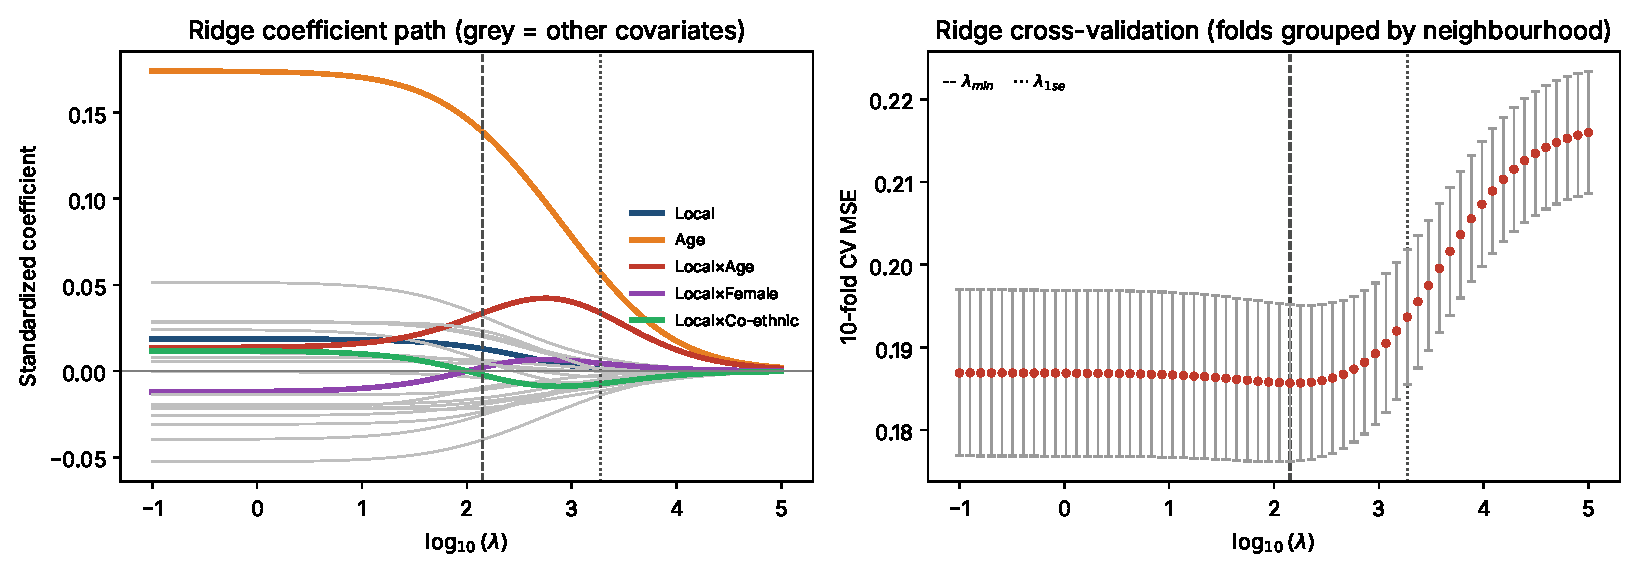
\includegraphics[width=\linewidth]{Figure1_Ridge.pdf}
\caption{Ridge: coefficient path (left) and 10-fold CV MSE with $\pm1$ SE bars (right). Outcome: Exempt; 23 standardized features (Local, 11 covariates, 11 Local$\times$covariate interactions); fixed effects and missing dummies partialled out. Dashed: $\lambda_{min}$; dotted: $\lambda_{1se}$.}
\end{figure}

\section{LASSO}
\begin{figure}[H]\centering
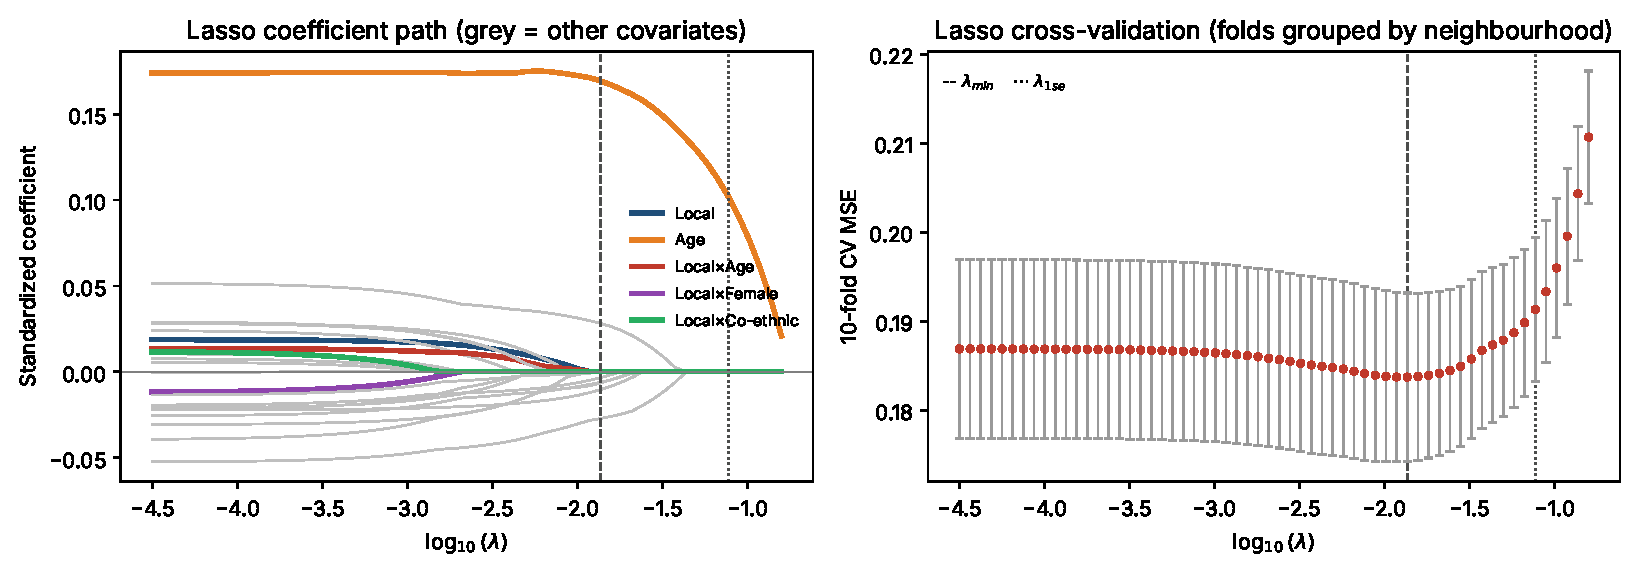
\includegraphics[width=\linewidth]{Figure2_Lasso.pdf}
\caption{Lasso: coefficient path (left) and 10-fold CV MSE with $\pm1$ SE bars (right). Same features, sample and folds as Figure 1.}
\end{figure}

\textbf{Findings.} All three models agree that \emph{age} is by far the strongest predictor of being exempted, while the Local treatment and its interactions are small: in OLS, Local raises exemptions for seniors by 7.5 pp ($p<0.05$) but not for widows, and no Local$\times$covariate term, including Local$\times$co-ethnic, is significant. Lasso sharpens this: at $\lambda_{min}$ it sets Local, Local$\times$Age and Local$\times$Co-ethnic to exactly zero (keeping only age, female, co-ethnic, assets and three tiny interactions), and at $\lambda_{1se}$ only age survives, so the heterogeneity terms add almost no predictive power. This tells us more than OLS alone: any favouritism by chiefs is too small or too non-linear to show up in linear interactions, which motivates the next step of estimating heterogeneity flexibly with a causal forest.

\end{document}
